\documentclass{article}

% if you need to pass options to natbib, use, e.g.:
\PassOptionsToPackage{numbers, square}{natbib}
% before loading neurips_2019

% ready for submission
% \usepackage{neurips_2019}

% to compile a preprint version, e.g., for submission to arXiv, add add the
% [preprint] option:
%     \usepackage[preprint]{neurips_2019}

% to compile a camera-ready version, add the [final] option, e.g.:
\usepackage[final]{neurips_2019}

% to avoid loading the natbib package, add option nonatbib:
%     \usepackage[nonatbib]{neurips_2019}

\usepackage[utf8]{inputenc} % allow utf-8 input
\usepackage[T1]{fontenc}    % use 8-bit T1 fonts
\usepackage{hyperref}       % hyperlinks
\usepackage{url}            % simple URL typesetting
\usepackage{booktabs}       % professional-quality tables
\usepackage{amsfonts}       % blackboard math symbols
\usepackage{nicefrac}       % compact symbols for 1/2, etc.
\usepackage{microtype}      % microtypography
\usepackage[english]{babel}
\usepackage{graphicx}
\usepackage{wrapfig}
\usepackage{amsmath}
\usepackage{bm}
\usepackage{subcaption}
\usepackage[title]{appendix}
\newcommand\tab[1][1cm]{\hspace*{#1}}


\title{Project 11: Mixture models for image classification}

% The \author macro works with any number of authors. There are two commands
% used to separate the names and addresses of multiple authors: \And and \AND.
%
% Using \And between authors leaves it to LaTeX to determine where to break the
% lines. Using \AND forces a line break at that point. So, if LaTeX puts 3 of 4
% authors names on the first line, and the last on the second line, try using
% \AND instead of \And before the third author name.

\author{%
  Nicholas Quek \\
  St Edmund's College\\
  University of Cambridge\\
  \texttt{nq212@cam.ac.uk} \\
}

\begin{document}
\maketitle

\begin{abstract}
Yelp released a photo dataset which is sorted into several arbitrary classes. These classes attempt to capture the restaurant's image and products. These classes facilitate Yelp's algorithms in selecting the best photos from the restaurants to aid in users' decision making. This paper proposes utilising topic modelling to generate groupings. These generated topics would capture the images' heuristics, exploiting their most discriminative features to group/differentiate them into topics. As expected, the proposed algorithm grouped the images differently from Yelp's categories. This paper utilised visualisation techniques, based on neural style learning, to obtain further insights on the generated topics. 
\end{abstract}

\section{Introduction}
Yelp is a business directory service and review site. Leveraging its social networking features, it crowd-sources text and photo reviews for businesses. Both restaurant customers and business owners have uploaded photo images to Yelp as part of reviews or as an advertising effort. Yelp has made available a dataset of these photos. It was originally put together for the Yelp Dataset Challenge which allows students to conduct research or analysis on Yelp's data and share their discoveries. The dataset is sorted into several predefined classes: "food", "drink", "menu", "outside" and "inside". 

Noise in the images can make automatic classification difficult. For example, most food images contain noise (things besides food), such as people, weather, plates, etc. However, human classification would readily classify these images under food. This paper attempts to investigate what classes naturally emerge from the semantic information of the photo images through the use of unsupervised topic modelling of features extracted using convolutional neural networks (CNN). The paper also attempts to visualise what these topics encapsulate and draw relations between these discovered topics to Yelp's predefined classes.

\section{Background}
The essence of this paper is an unsupervised image classification problem. CNNs are typically used when interacting with images. CNNs are often used in conjecture with fully-connected layers. which would be tuned to perform a specific task. Traditionally, the entire machine learning models would have to be rebuilt from scratch if the task it is trying to perform changes.  

Transfer learning overcomes this isolated learning paradigm. The knowledge captured by CNN models on one task could be applied to another task. Therefore, we construct CNNs on a huge dataset with a diverse distribution of images (e.g. ImageNet \cite{imagenet}). The model is expected to have learned a robust set of features \cite{vgg}, which are spatial, rotation, and translation invariant. The model is then used as a feature extractor to produce inputs for subsequent models such as a classifier. The ability to extract features from new datasets without additional training makes machine learning techniques which were previously infeasible on certain datasets possible. 

This paper attempts to use topic modelling, a primarily text-specific technique, to images. This technique is made feasible by having a pre-trained CNN functioning as a feature extractor. The CNN converts an image (a 3-dimensional entity) into a vector of features. Topic modelling works on these vectors and attempts to cluster the images into several topics.

\subsection{Convolutional Neural Networks}
Convolutional Neural Networks (CNNs) are a category of feed-forward neural networks, commonly used in the image domain. Due to the three-dimensional nature (width, height and colour) of images, ordinary neural networks typically have problems scaling to the entire image and will encounter overfitting problems during training. CNN differs from traditional neural networks by using a 3-dimensional volume of neurons. Neurons in each layer are only connected to a small region of the layer before it, forming filters. These filters allow the CNN to successfully capture the spatial and temporal dependencies in images. The usage of filters results in a reduction in the number of tunable parameters and re-usability of weights. This allows CNN to be trained more easily than traditional neural network while avoiding overfitting problems \cite{cnn1}.

A typical architecture comprises of a number of convolutional and subsampling layers followed by pooling layers and fully connected layers. The capacity of a CNN can be controlled by varying the depth and breadth of the architecture. Much research had been done in the field of CNNs to discover the best configurations for specific tasks. 

For this paper, we would be using a pre-trained CNN, VGGNet \cite{vgg} for extraction of features from images. VGGNet was introduced by the Visual Geometry Group from the University of Oxford. VGGNet was the winner of the ImageNet Large Scale Visual Recognition Competition (ILSVRC) 2014 in the localization task and 1st runner-up in the classification task. The pre-trained VGG 19-layer model with batch normalization is used for this paper. 

\begin{figure}[h]
  \centering
  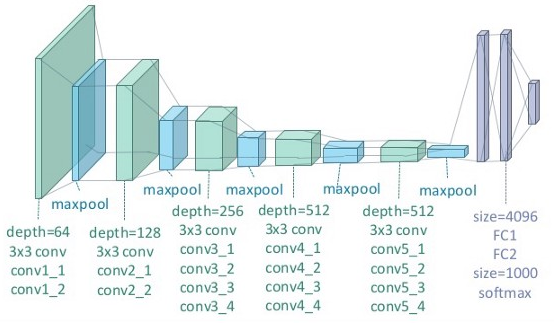
\includegraphics[width=8cm]{vgg19.png}
  \caption{VGG-19 Architecture \cite{vgg19img}}
  \label{vgg_architecture}
\end{figure}

Figure \ref{vgg_architecture} is a visual representation of the VGG-19 architecture. VGG-19 takes a fixed-size 224 x 224 RGB image as input. The image is preprocessed, normalised using the mean and standard deviation of the RGB values, computed on every pixel in the training set. The image is passed through two convolutional layers composed of filters with a very small (3 x 3 pixel) receptive field. After these convolutional layers, spatial pooling is carried out. Max-pooling is performed over a 2 x 2 pixel window, with stride 2. Multiple repetitions of convolution and max-pooling are carried out. During each iteration, the number and depth of convolutional layers before max-pooling changes. After five iterations, there are three fully-connected layers followed by a soft-max layer. 

\subsection{Categorical Mixture Models}
A mixture model corresponds to a mixture distribution which contains a collection of random variables. A random variable is initially selected from the collection according to given probabilities of selection. The value of the selected random variable is then realised. Categorical Mixture Models are a sub-family of mixture models which are described by discrete probability distributions, where a random variable can take one of the possible K categories.   

Categorical Mixture Models have been commonly applied in topic modelling. The Latent Dirichlet Allocation \cite{LDA} model allows documents to be associated with multiple topics. The Topics over Time \cite{ToT} model allow for distribution over topics conditioned on time. In this paper, the simple mixture-of-multinomials model (described in Figure \ref{CMM}) is used.  

\begin{figure}[]
  \centering
  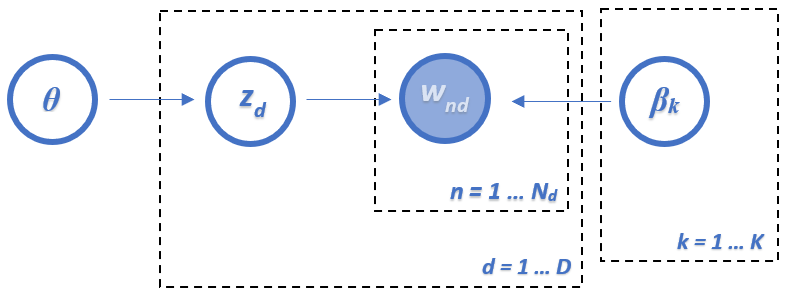
\includegraphics[width=10cm]{CMM.png}
  \caption{Mixture-of-multinomial Model}
  \label{CMM}
\end{figure}

We assume that a document belongs to one of the $K$ possible topics. A document is composed of $N_d$ different words from a vocabulary of size $M$. The distribution of words could be modelled as a mixture of $K$ different $M$-dimensional categorical distributions, $\{\beta_1,\ldots,\beta_K\}$. 

The process of generating a corpus is as follows:
\begin{enumerate}
    \item For each document $d$, pick a topic $z_d \in \{1,\ldots, K\}$ from a multinomial distribution $\theta$ 
    \item For each word token $w_{nd}$ in document $d$, pick word $w_{nd}$ from the multinomial distribution $\beta_{z_d}$ of the document's assigned topic.
\end{enumerate}



\section{Methodology}
For this paper, the simple mixture-of-multinomials model is used. It is a two-level hierarchical model, in which the corpus is represented as random mixtures over latent topics where each document is assigned a topic. Each topic is characterized by a distribution over words. 

Since we are applying techniques used in the text domain to images, we need to define an analogy between their respective terminologies as follows:
\begin{enumerate}
    \item A corpus, $D$ is an image data set.
    \item A document, $d \in D$ is equivalent to an image.
    \item A word, $w_{nd}$ corresponds to an extracted top-level feature of the convolution layer from the image corresponding to document $d$.
\end{enumerate}

\subsection{Preparing the corpus}
The Yelp dataset contains a total of 200,000 photos. The images belong to five broad classes: drink, food, menu, inside and outside. Table \ref{tab:images} captures the class distribution of these images. The dataset is dominated by images of food, with a significant portion being images of restaurant interiors. 

\begin{table}[h]
  \caption{Distribution of images}
  \label{tab:images}
  \centering
    \begin{tabular}{|c|c|c|c|c|}
    \hline
 Drink & Food & Menu & Inside & Outside \\ \hline
 18121 (9\%) & 114874 (57\%) & 3023 (2\%) & 52448 (26\%) & 11534 (6\%)  \\
 \hline
    \end{tabular}
\end{table}

There is no uniformity in image size, ranging from 150 x 150 pixels to 600 x 600 pixels. To handle the variants in size, some preprocessing was performed to get the images into the appropriate format VGGNet requires as its input. The images are first resized to 256 x 256 pixels. After which, a centre crop is performed to obtain a 224 x 224 pixel image. The obtained image is then normalised using the mean and standard deviation of the RGB values, computed on every pixel in the ImageNet training set which VGGNet was originally trained on. The means are 0.485, 0.456 and 0.406 and standard deviation are 0.229, 0.224 and 0.225 for the RGB channels respectively. 

\subsection{Extracting features from images}\label{extract}
After pre-processing, we can now extract features from the images. A word in our model corresponds to an extracted top-level feature from the CNN. There are two options commonly used for feature extraction. The first is the ante-penultimate layer. The second is the last convolution layer. While there are many other options, they tend to perform poorly as features. For example, the last layer (before softmax) of VGG-19 can be regarded as a linear classifier, classifying images into the ImageNet classes. However, this layer is often too overfitted for the specific task for usage in other tasks. In the last convolution layer, the low-level features are extracted. In a topic modelling task, it might be more sensible to work with lower-level features. Low-level features are to images what words are to documents. The output from the last convolution layer is a tensor of 512 x 7 x 7. 

This paper explores multiple ways to convert these features into `words'.

\subsubsection{Repeated Words using Sub-tensors}\label{repeatedSubtensor}
The tensor is split into 512 sub-tensors. The size of the vocabulary is 512. Each sub-tensor correspond to a word in the vocabulary, and they contain 49 (7 x 7) values each. A word is considered to be in the image if a value is above a pre-determined activation threshold. There can be a total of 49 repeated words. This approach attempts to aggregate the lower-level features within each sub-tensors.

\subsubsection{Sub-tensors Means}\label{meanSubtensor}
Similar to Section \ref{repeatedSubtensor}, this approach aggregates the lower-level features from a different perspective. The tensor is split into 512 sub-tensors and each sub-tensor correspond to a word in the 512-sized vocabulary. The difference is that the word is in the image if the mean of the sub-tensor is above a pre-determined activation threshold.

\subsubsection{Repeated Words using Sub-tensor Means}\label{repeatedmeanSubtensor}
The approach is similar to Section \ref{meanSubtensor}. The number of occurrences of the word is the value of the mean of the sub-tensor divided by the pre-determined activation threshold. This means that a feature which is strongly activated would have multiple occurrences as words. 

\subsection{Gibbs Sampling}
Having extracted the features, we now have a complete analogy to text-based topic modelling, allowing us to apply the simple mixture-of-multinomials model. In order to model the topics, the Dirichlet distribution is chosen as the prior to describe the multinomial distributions. \\
\newline
\tab $\theta \sim Dir(\alpha)$ is a symmetric Dirichlet distribution over topic probabilities \\
\\
\tab $\beta_k \sim Dir(\gamma)$ is a symmetric Dirichlet distribution over vocabulary probabilities \\

In the model, there are three types of variables $\theta, \beta_k, z_d$ which needs to be sampled. The joint distribution is intractable therefore making direct sampling difficult if not impossible. However, we can utilise Gibbs sampling, a Markov chain Monte Carlo algorithm, which eventually generates dependent samples from the joint distribution if performed properly. We iteratively sample from one of the three types of variables while conditioning on all the other variables.

The M-dimensional categorical distributions for words,
$$p(\beta_k|\bm{w}, \bm{z}) \propto p(\beta_k)\prod_{d:z_d=k}p(\bm{w}_d|\beta_k)$$

The topic label assignments for each document,
$$p(z_d = k|\bm{w}_d, \bm{\theta}, \bm{\beta}) \propto \theta_k p(\bm{w}_d|\beta_{k})$$

The multinomial topic distribution,
$$p(\theta|\bm{z}, \alpha) \propto p(\theta|\alpha) p(\bm{z}|\theta) \propto Dir(\bm{c}+\alpha)$$
where $c_k = \sum_{d:z_d=k} 1$ are counts for mixture $k$.

\subsubsection{Collapsed Gibbs Sampling}
A neat technique we can perform to simplify the process is collapsed Gibbs sampling. We can marginalise over $\theta$
$$p(z_d = k | \bm{z_{-d}}, \alpha) = \dfrac{\alpha + c_{-d,k}}{\sum_{j=1}^K \alpha + c_{-d,j}}$$
where index $-d$ means all except $d$, and $c_k$ are counts of words occurrences in topic $k$.

Therefore, the latent topic assignments becomes
$$p(z_d = k | \bm{w}_d, \bm{z_{-d}}, \bm{\beta},\alpha) \propto p(\bm{w}_d | \beta_k) \dfrac{\alpha + c_{-d,k}}{\sum_{j=1}^K \alpha + c_{-d,j}}$$

In each sweep of the Gibbs sampler, we iterate through every document. For each document, we remove the word counts of the document from the initial assigned topic. We compute the latent probability and sample it to re-assign a topic to the document. After the assignment, we add the word counts of the documents to the new topic and move on to the next document. By marginalising over $\theta$, we made the topic assignments dependent on each other. Each sweep of the Gibbs sampler produces a sample of topic assignments for the documents, and this sample induces a posterior predictive distribution for the probability of each topic. 

\section{Experiments}
\subsection{Data setup}
A held-out test set comprising of 10\% of the entire Yelp dataset is reserved, split using stratified means to preserve the class distributions. The remaining data is used for training and validation. We apply five-fold stratified cross-validation to the remaining data, using 80\% of the images for training and 20\% for validation. 

\subsubsection{Inferring Posterior Predictive Distributions}

\begin{wrapfigure}[13]{r}{5cm}
  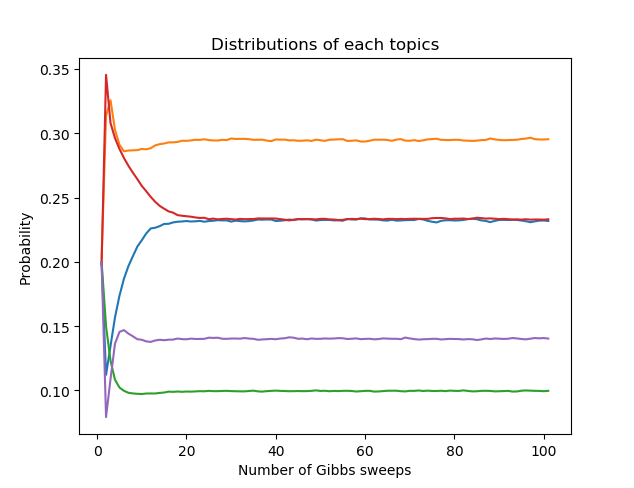
\includegraphics[width=5cm]{convergence.png}
  \caption{Topic distributions of the Gibbs Sampler}
  \label{convergence}
\end{wrapfigure}

The Gibbs sampler was run on the training data. Typically, samples from the beginning of the Gibbs sampler do not accurately describe the joint distribution. In order to perform burn-in (removal of these samples), we observe the behaviour of the Gibbs sampler. Figure \ref{convergence} shows the topic distributions as a function of the number of Gibbs sweeps for the repeated words using sub-tensor means approach. 

The topic distributions appear to converge after 40 iterations. Therefore, we ignore the initial 40 samples to ensure that the samples taken are from the joint distribution. We averaged over the samples to infer the posterior predictive distributions over topics and words. This was performed for all the three stated approaches in Section \ref{extract}.

\subsection{Perplexity}
Having inferred both the topic distribution, $\theta$ and word distribution, $\bm{\beta}$, we now need a metric to compare between the various approaches. In text modelling, model performance is often evaluated in terms of per word perplexity. Perplexity measures how well a probability distribution or probability model predicts a sample. A low perplexity indicates that the probability distribution is good at predicting the sample, as it is less surprised by the sample.  

The perplexity for a document is given by $exp(-\ell/n)$ where $\ell$ is log joint probability over the words in the document.

\vspace{-0.5cm}
\begin{equation}
\begin{split}
\ell_d &= p(\bm{w}_d | \theta, \bm{\beta}) \\
 & = \sum_k^K \frac{dc_k + \alpha}{\sum_i^K dc_i + \alpha}\prod_{n=1}^{N_d} \frac{c_{w_{nd}}^k + \gamma}{\sum_{m=1}^M c_m^k + \gamma}
\end{split}
\end{equation}
where $dc_k$ is the count of documents assigned to topic $k$ in the training set and $c_m^k$ is the count of the word $m$ from the training data, assigned to topic $k$. 

\subsection{Parameter Tuning} \label{params}
Multiple tests were performed using different activation level, $\alpha$ and $\gamma$. The posterior predictive topic and word distributions inferred during training are applied to the validation set to compute the per word perplexity. Five-fold validation was performed and the average perplexity scores were used to select the hyper-parameters. For the three different approaches, the models performed best when $\alpha$ and $\gamma$ are small (10.0 and 1.0 respectively) and the activation level was large (1.5 and 0.3 for the means), but not large enough to have `documents' without `words'. Table \ref{tab:perplexity} displays the per word perplexity score for the different approaches. 

\begin{table}[h]
\caption{Per Word Perplexity Scores}
\label{tab:perplexity}
\centering
\begin{tabular}{|c|c|}
\hline
Approach                              & \multicolumn{1}{l|}{Per Word Perplexity} \\ \hline
Repeated Words using Sub-tensors      & 394.6                                    \\
Sub-tensors Means                     & 343.5                                    \\
Repeated Words using Sub-tensor Means & 330.7                                    \\ \hline
\end{tabular}
\end{table}

The repeated words using sub-tensors approach performed the worst. By considering each value in the sub-tensor as a possible word, we are introducing noise into the equation. The other approaches are able to reduce the noise by aggregating the values in the sub-tensors. The repeated words using sub-tensor means approach achieved the lowest perplexity score. This approach places more weight on larger sub-tensor means. Essentially suppressing low-valued sub-tensors, reducing the overall noise. Therefore, this approach was chosen to evaluate the test data. 

\section{Evaluation}
The repeated words using sub-tensor means approach achieved the lowest perplexity score on the validation set, which meant that the approach generated models which can best predict the samples in the validation set among the attempted approaches. Using the hyper-parameters found in Section \ref{params}, the best performing model from the five-fold cross-validation is chosen to evaluate the test data. The selected model achieved a per word perplexity score of 331.17 and is also used to organise the images in the held-out test set into five topics. 

With the Yelp's class labels, we use a confusion matrix to analyse the model performance. An overview of the performance of the models is given by the two confusion matrices presented in Figure \ref{img:confusion}. In both matrices, the rows are ground truth classes, and columns are the topics generated by the model. Figure \ref{confusionleft} shows the percentage of the labelled images captured by each topic. This matrix provides insight into how a specific class is distributed across the topics. A large value would indicate that most of the images labelled with the class are captured by the topic. Figure \ref{confusionright} displays the percentage of labels within each topic. It captures the distribution of each class in a topic.

\begin{figure}
\centering
\subcaptionbox{Percentage of topics in each label\label{confusionleft}}
{%
    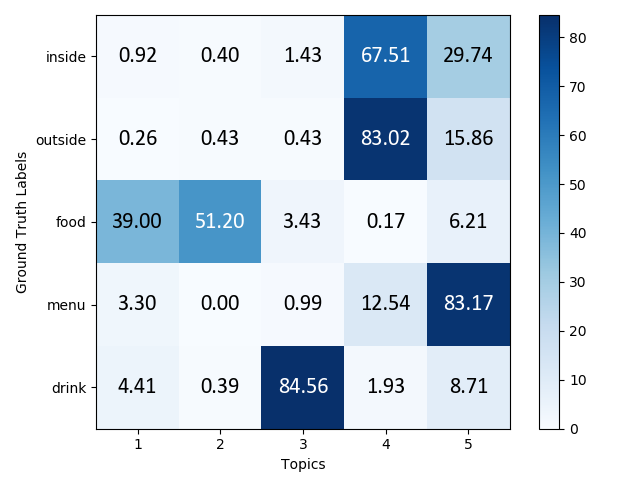
\includegraphics[width=7cm]{confusiona.png}
    \hspace{0.02\columnwidth}
}%
\subcaptionbox{Percentage of labels in each topic\label{confusionright}}
{%
    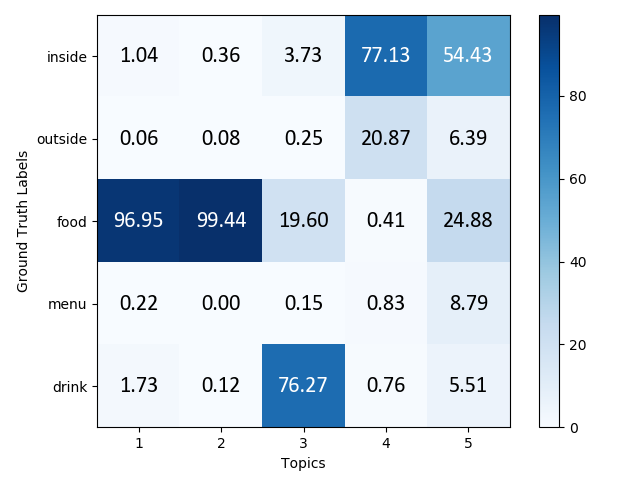
\includegraphics[width=7cm]{confusionb.png}
    \hspace*{\fill}
}%
\caption{Image distribution of the Repeated word using sub-tensor means approach} \label{img:confusion}
\end{figure}

From Figure \ref{confusionright}, we notice that almost everything under Topic 1 and 2 was labelled as food images. The two topics are likely capturing some subcategories of food. By referring to Figure \ref{confusionleft}, 90.2\% of all food images ended up under Topic 1 and 2. Therefore, the subcategories of food which are captured by the two topics span the bulk of the food category.

Topic 3 captures a significant portion of drinks. 84.56\% of all images labelled drink were gathered under Topic 3. However, not all the images in Topic 3 are from drinks. 76.27\% of the topic are from drinks while the other images are from food. Since most drinks were captured, it is safe to deduce that Topic 3 is capturing liquid-related features. Given that it captures a portion of food images, a possible deduction is that Topic 3 also captures food products with liquids, such as stews and soups.

Topic 4 largely captures both inside and outside. It is likely capturing features related to the restaurant environment such as people, plants and tableware. 

Interpretation of Topic 5 is not as straightforward as the others. The topic has the majority of its images labelled inside, with a large portion of food. However, a key characteristic is that the topic captures a significant portion of images labelled menu. A possible interpretation is that it is capturing restaurant interiors, such as tables and menus, which commonly appears in images of these three classes.

\section{Visualisation of Modelled Topics}
A common strategy to better understand the generated topics is to observe the top few words in the topic and derive any similarities between them. However, in the case of this paper, the `words' in the topics are features extracted by the CNN, which would not be understandable to a human observer. Therefore, this paper attempts to visualise the features extracted by the CNN. 

\subsection{Visualisation process}
The exact way neural networks see and interpret the world remains a black box. However, we do have an understanding of how they recognize specific patterns or objects. When a specific pattern which the network is trained to recognise appears, a certain feature map within the network would be activated \cite{visualcnn}. 

The visualisation strategy for a certain feature map would be to generate a pattern by optimizing the pixel values in a random image. To do that, we fix the network weights. The network will not be trained. Instead, we adopt an idea used in neural style transfer \cite{nstyletransfer}. We start with a random image. Passing the image through the network will reveal the activation of the feature, which allows for the gradients with respect to the input image pixels to be calculated. We proceed to perform gradient descent optimisation on the pixel values such that the activation of the chosen feature is maximised.

Unfortunately, the resulting visualisation is dominated by high-frequency patterns. It was discovered that the frequency of the desired pattern appears to increase with the image size. This is likely due to the fixed size convolutional  filters. Their relative size compared to the image changes the frequency of the patterns. By increasing the image size, the relative size of the generated pattern will reduce and the pattern frequency increases. For an ideal visualisation, a low-frequency pattern with high resolution is preferred. For the visualisations, we start with a small random image. After pixel values were optimized for multiple epochs, the image is upscaled by a pre-determined factor. To further reduce high-frequency patterns, the images are blurred after upscaling. Multiple iterations were performed to obtain the visualisation.

The final result is a low-frequency pattern in a higher resolution without too much noise. The final image cannot be generated by directly optimising the pixel values. The process of optimising followed by upscaling provides a starting point which produces a clearer image and helps to avoid poor local minima. 

\subsection{Visualised Topics}
The hyper-parameters for the visualisation process is determined using a grid search. The optimal parameters are selected based on the clarity of the produced pattern. The most popular words of Topic 3 were examined. Figure \ref{feat342} shows the second most common word in Topic 3. The feature map seems to capture can-like objects, which agrees with the theme of drinks which Topic 3 represents.

Figure \ref{img:Topic5feat} shows the more interpretable features of Topic 5. Figure \ref{feat478} appears to capture the humanoid figure. Hence, humans make up a significant portion of the meaning of Topic 5. Rectangular objects activated the feature map in Figure \ref{feat413}. This feature is likely responsible for capturing the images labelled menu, as menus tend to be rectangular.

\begin{figure}[h]
\centering
\subcaptionbox{Feature Map 342\label{feat342}}
{%
    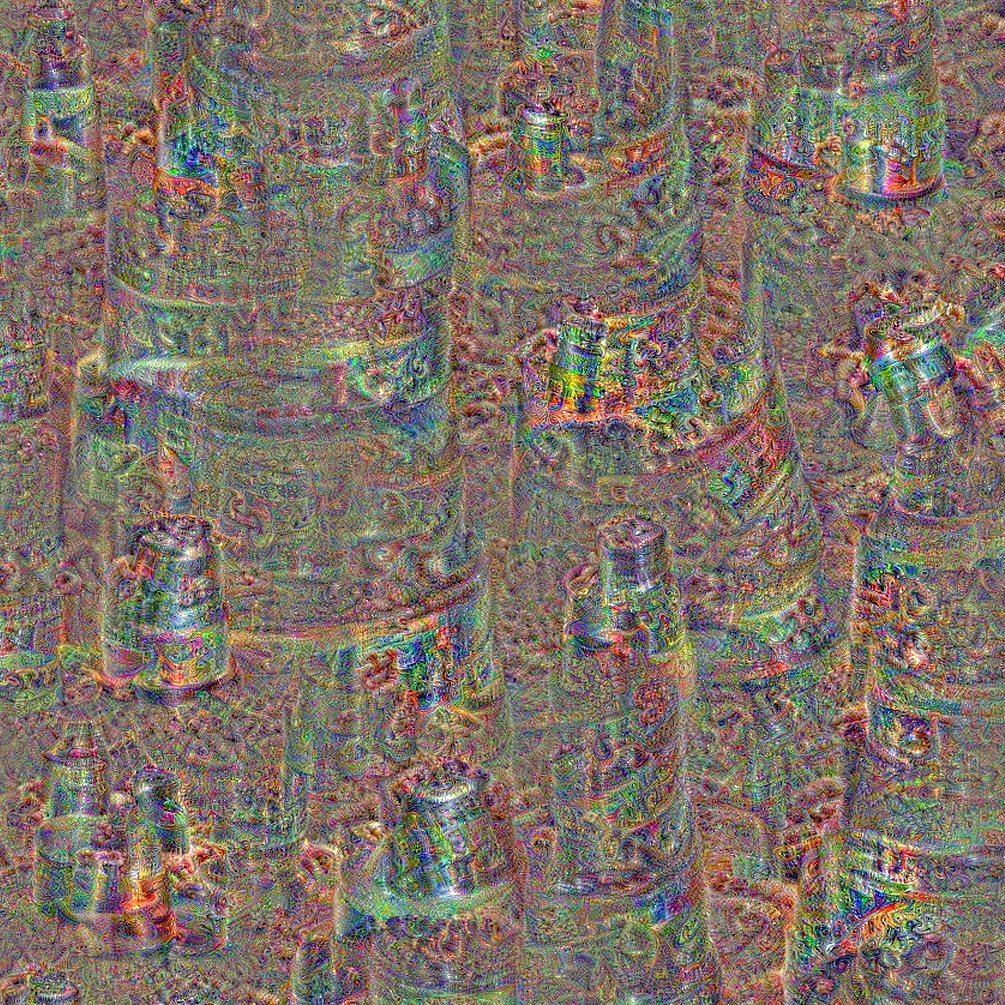
\includegraphics[width=4cm]{342.jpg}
    \hspace{0.04\columnwidth}
}%
\subcaptionbox{Feature Map 478\label{feat478}}
{%
    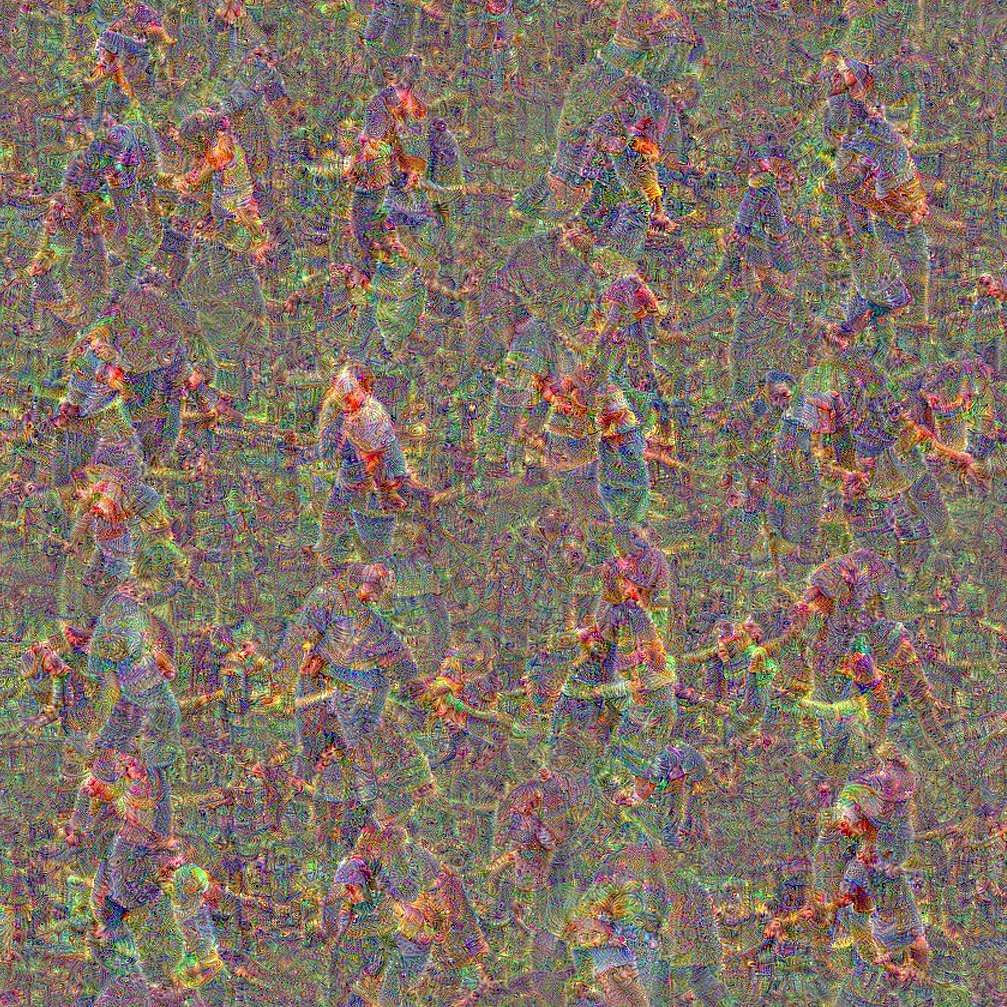
\includegraphics[width=4cm]{478.jpg}
    \hspace{0.04\columnwidth}
}%
\subcaptionbox{Feature Map 413\label{feat413}}
{%
    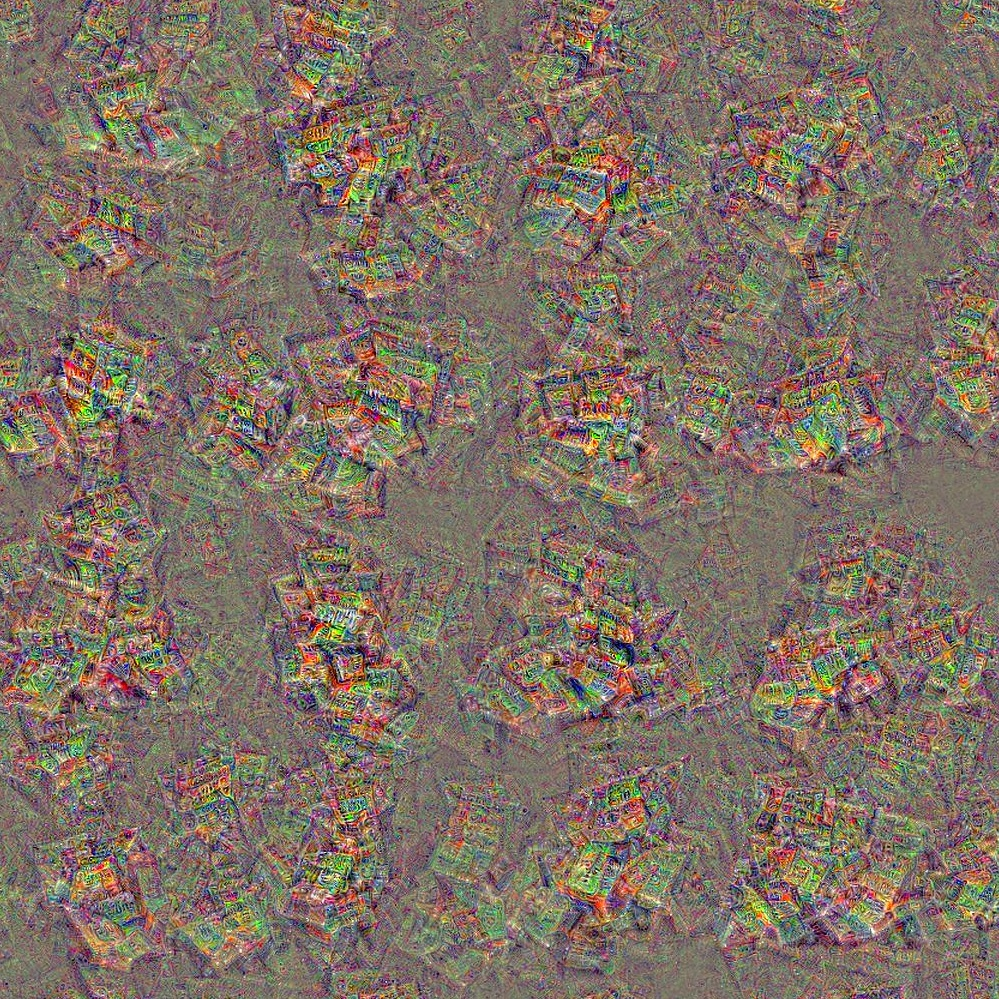
\includegraphics[width=4cm]{413.jpg}
    \hspace*{\fill}
}%
\caption{Visualised Feature Maps} \label{img:Topic5feat}
\end{figure}

The top 5 features for each topic can be found in Appendix \ref{AppendixVisualisation}. However, not all the features are clear and straightforward. Many are also subjected to personal interpretation, which would include bias and prior beliefs of the meaning of the topics.  
\section{Future Work}
This paper focused primarily on extracting features from the last convolutional layer. However, this is not the only layer for feature extraction. Future work can experiment with other options such as the ante-penultimate layer which generally also have useful extracted features. Comparisons between these models would be tricky as perplexity is less useful when the cardinality of the generated vocabulary is different. Other methods of comparisons such as Pointwise Mutual Information would have to be employed to determine the better model.

The paper uses the simple mixture-of-multinomials model to relate the Yelp pre-defined classes with the generated topics. However, other categorical mixture models can be applied depending on the intent. For example, Latent Dirichlet Allocation could be utilised for unsupervised tagging of images. The images in the dataset are not isolated but often contain a mixture of different objects. An image of burgers may contain a human posing with the burger. An unsupervised approach to tagging would leverage inherent heuristics and produce more discriminative tags compared to the traditional approach of generating tags. 

\section{Conclusion}
This paper utilised topic modelling, a technique commonly used in the text domain, on images. The images are grouped with the features extracted using a pre-trained CNN, VGG-19. The generated topics capture the inherent characteristics within the images and are mostly different from the original Yelp's classes. Two of the generated topics are subcategories of the food class. One topic captures liquid-related features while another capture features relating to the restaurant environment. The final topic was less interpretable. A visualisation technique was employed in an attempt to gain insight into this final topic. The top features capture humanoid and rectangular objects, which contribute to our understanding of the final topic. All code used in this paper can be found in Github\footnote{https://github.com/Kocolipy/ImageMixtureModel}.

\bibliographystyle{unsrt}
\bibliography{sample}

\newpage
\begin{appendices}
\section{Topic Visualisations}\label{AppendixVisualisation}
The top five features of each topics were visualised and displayed beginning from the left.

\begin{figure}[h]
\centering
\subcaptionbox{Topic 1\label{tp_1}}{%
  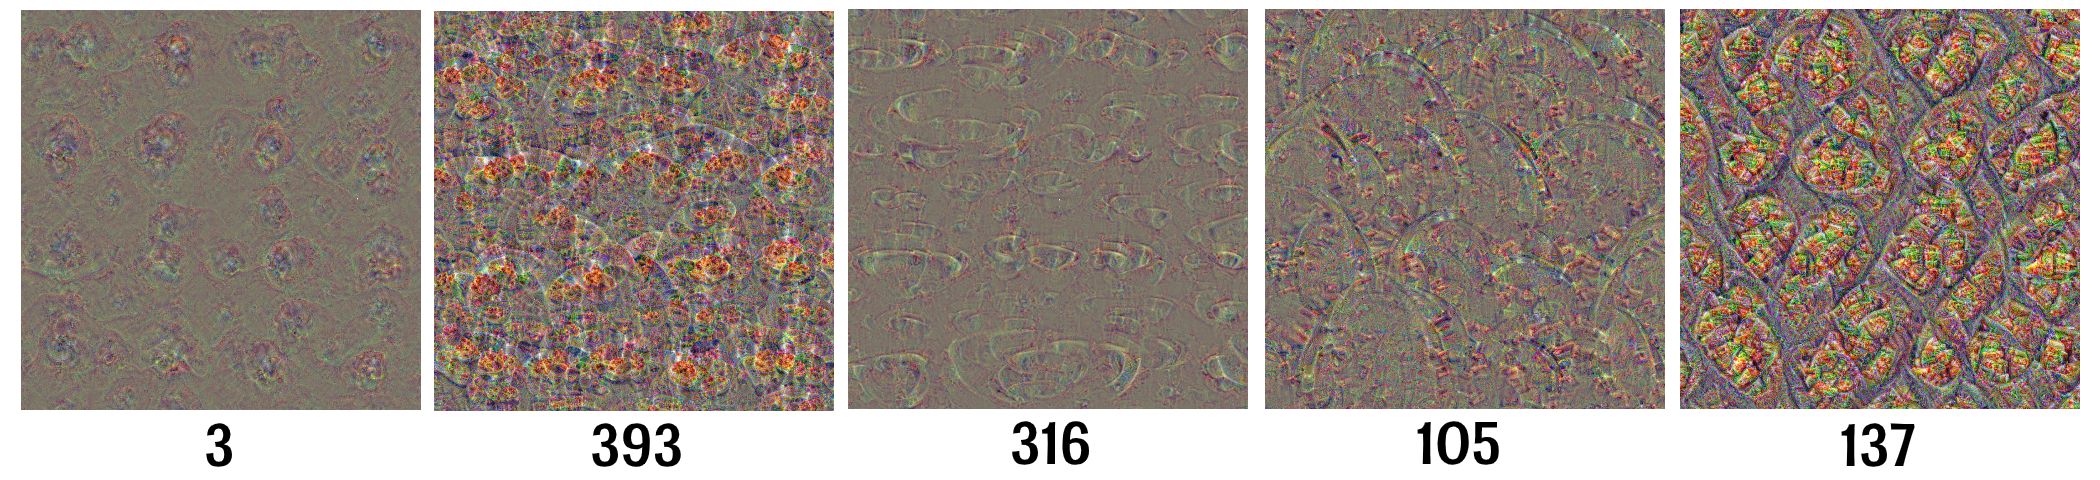
\includegraphics[width=14.2cm]{Topic1.png}%
  }\par\medskip
\subcaptionbox{Topic 2\label{tp_2}}{%
  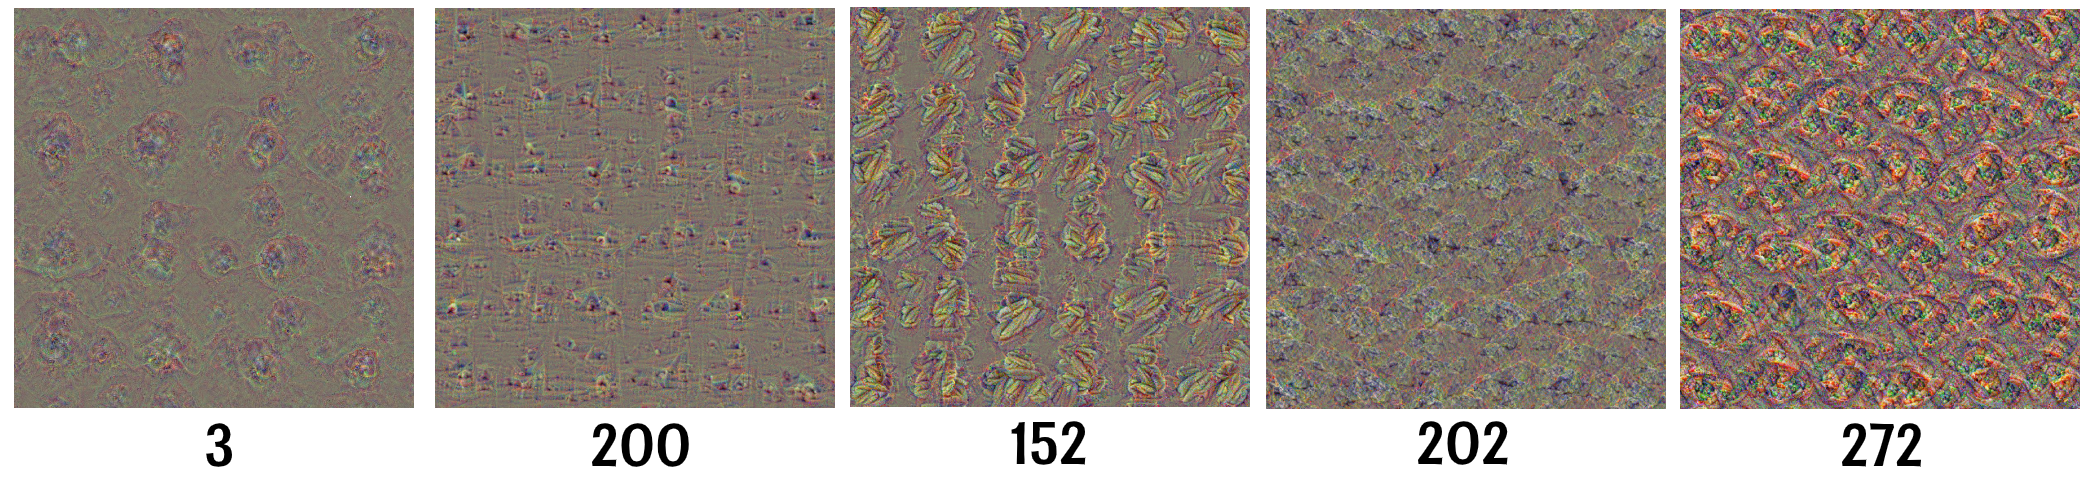
\includegraphics[width=14.2cm]{Topic2.png}%
  }\par\medskip    
\subcaptionbox{Topic 3\label{tp_3}}{%
  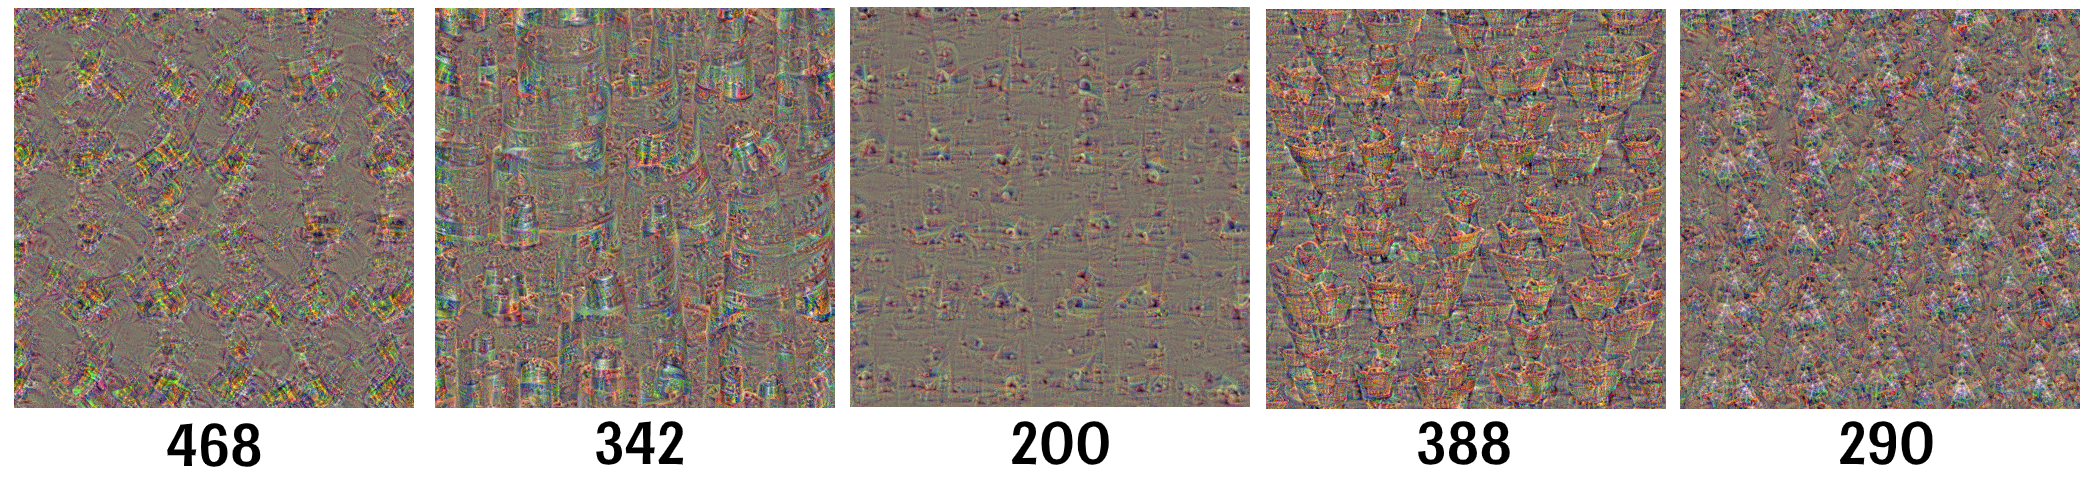
\includegraphics[width=14.2cm]{Topic3.png}%
  }\par\medskip        
\subcaptionbox{Topic 4\label{tp_4}}{%
  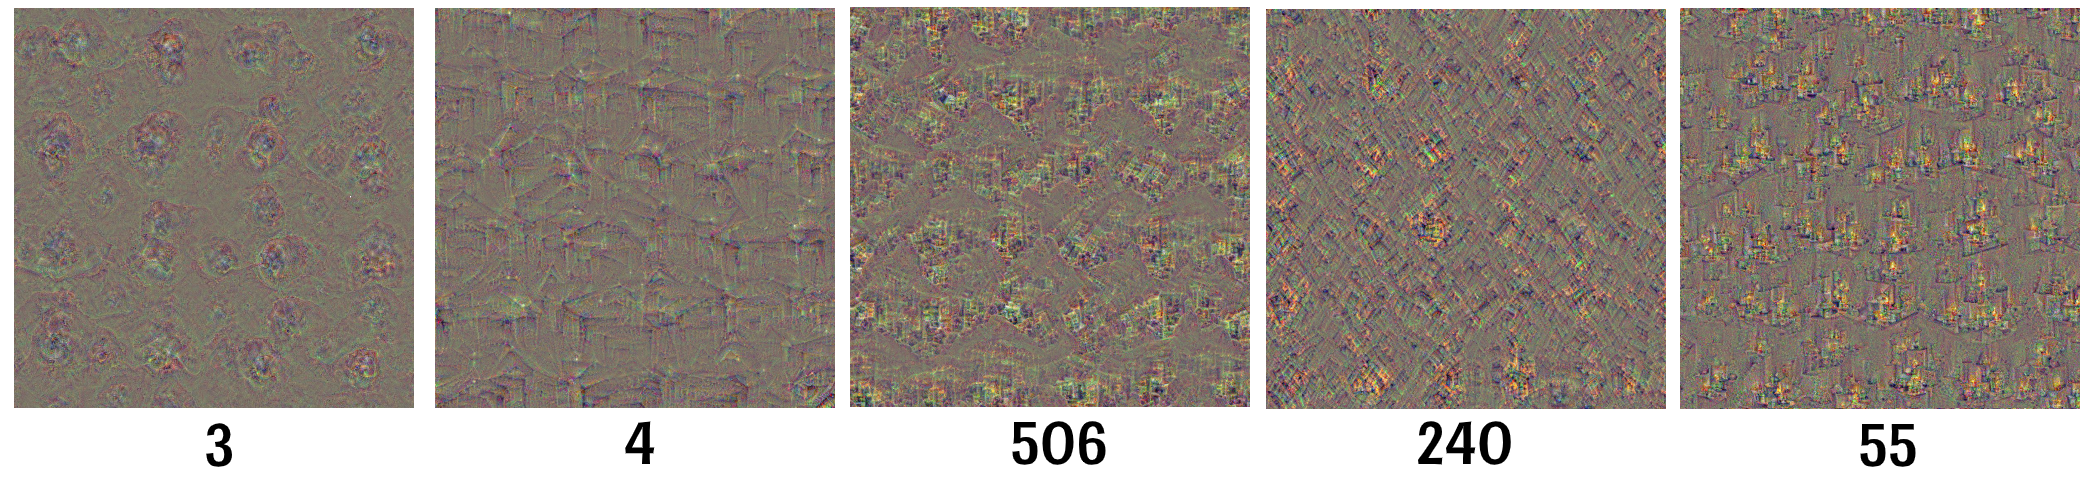
\includegraphics[width=14.2cm]{Topic4.png}%
  }\par\medskip            
\subcaptionbox{Topic 5\label{tp_5}}{%
  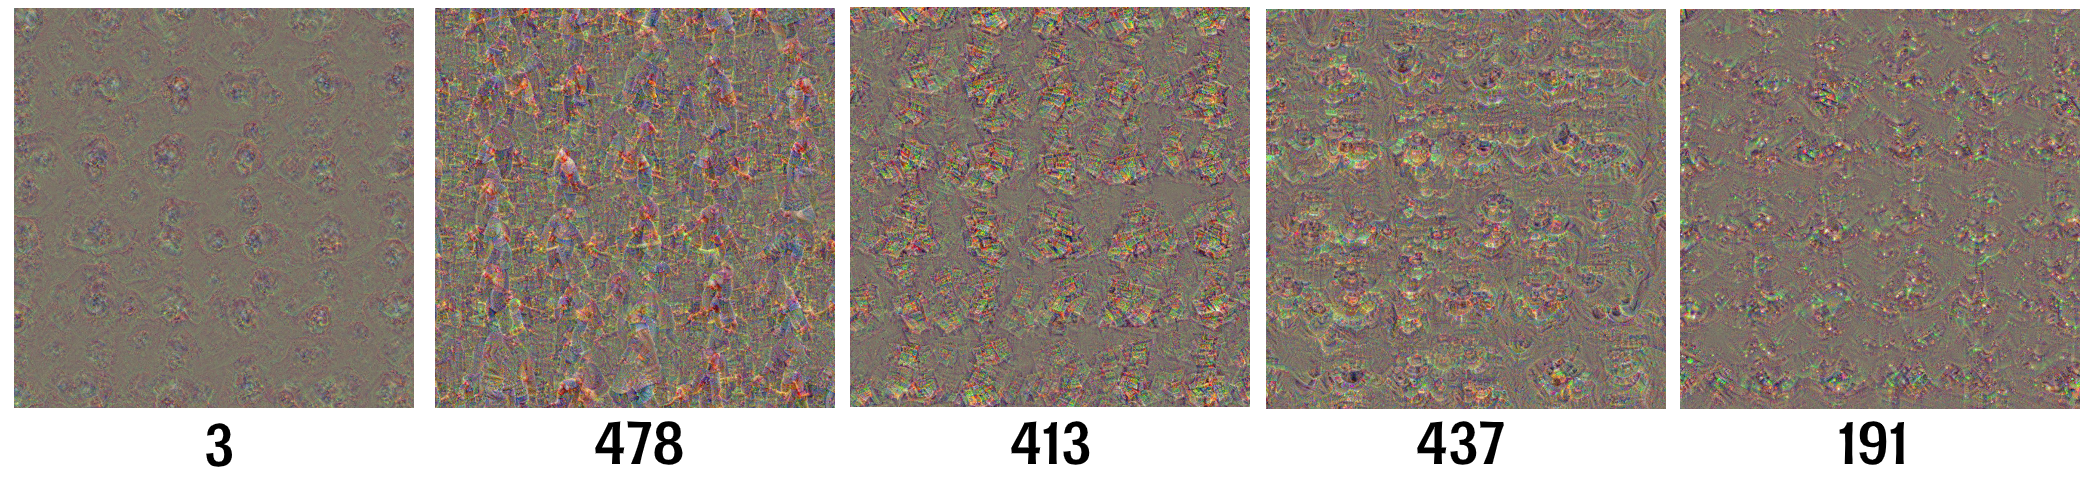
\includegraphics[width=14.2cm]{Topic5.png}%
  }

\label{TS}
\end{figure}
\end{appendices}

\end{document}
